%! Author = chaorn
%! Date = 13.08.24

\subsection{Fuzzing mit boofuzz}\label{subsec:boofuzz}
In dem folgenden Kapitel wird das Aufsetzen der Testumgebung und die darin durchgeführten Experimente mit dem Fuzzing-Tool
boofuzz beschrieben.
\subsubsection{Setup}
Zur Entwicklung einer Fuzzing-Kampagne mit boofuzz sind mehrere Schritte erforderlich.
Zunächst muss das Zielsystem identifiziert und analysiert werden, um die relevanten Protokollspezifikationen und
Kommunikationsmuster zu verstehen.
Darauf aufbauend werden die Testfälle definiert, die die verschiedenen Protokollfelder und Eingabeparameter abdecken sollen.
Die Testfälle werden in boofuzz als \textit{Fuzz-Template} definiert, das die Struktur und den Inhalt der zu füllenden
Nachrichten beschreibt.
Das Fuzz-Template besteht aus einer Reihe von Feldern, die die verschiedenen Teile der Nachricht repräsentieren, wie z.B.\ den
Fixed Header, den Variable Header und den Payload bei \gls{mqtt}-Nachrichten.
Jedes Feld kann verschiedene Eigenschaften wie den Typ, die Länge und den Wertebereich der Eingabe enthalten.
In dem Fall der \gls{mqtt}-Nachrichten können die Felder z.B.\ den Steuerpakettyp, die QoS-Ebene und den Topic-Namen,
wie in Kapitel~\ref{subsec:mosquitto-mqtt} beschrieben, repräsentieren.
Hierbei ist es wichtig, die Protokollspezifikationen und die erwarteten Eingabewerte zu berücksichtigen, um realistische
Testfälle zu erstellen.
Nachdem die Testfälle definiert sind, wird eine Fuzzing-Kampagne gestartet, bei der boofuzz automatisch eine Vielzahl
von zufälligen oder systematischen Eingaben generiert und an das Zielsystem sendet.
Während des Fuzzings kann boofuzz den Zustand des Zielsystems überwachen und auf unerwartete Ereignisse wie Abstürze oder
Fehler reagieren.
Dieser Schritt ist jedoch nicht standardmäßig eingebaut und muss vom Benutzer implementiert werden.
Die Implementierung der Reaktion auf unerwartete Ereignisse kann z.B.\ das Neustarten des Zielsystems, das Anpassen der
Fuzzing-Strategie oder das Protokollieren von Fehlern umfassen und erfolgt über ein in boofuzz implementiertes Interface.
Dieses Interface beinhaltet die Monitor-Klassen \texttt{ProcessMonitor, NetworkMonitor} und \texttt{CallbackMonitor}.
Die \texttt{ProcessMonitor}-Klasse überwacht den Zustand des Zielsystems, indem sie den Prozessstatus überwacht und auf
Abstürze oder Fehler reagiert.
Dieser Monitor wurde zum Beispiel in der Analyse des \gls{mqtt}-Brokers Mosquitto verwendet, um auf Abstürze des Brokers
zu reagieren und die in den Abstürzen enthaltene debug-Informationen abzugreifen und zu speichern.
\newline\newline
Eine in dieser Arbeit verwendete Kernkomponente von boofuzz ist die Option ein Feld als \texttt{fuzzable} zu definieren.
Ein \texttt{fuzzable} Feld ist ein Feld, das zufällig generierte Eingaben erhalten darf und somit für das Fuzzing relevant ist.
Mit dieser Option können Testfälle erstellt werden, die systematisch verschiedene Eingaben in bestimmte Felder einfügen,
um präzisere und effektivere Fuzzing-Kampagnen durchzuführen.
Die \texttt{fuzzable}-Option ermöglicht es, die Eingaben gezielt zu steuern und bestimmte Protokollfelder oder Eingabeparameter
zu testen, um potenzielle Schwachstellen zu identifizieren.
Gerade im Fall von \gls{mqtt}-Nachrichten ist es wichtig, die verschiedenen Felder wie den Fixed Header, den Variable Header
und den Payload systematisch zu füllen.
\newline\newline
Für das Entwickeln einer Fuzzing-Kampagne wurden im Rahmen dieser Arbeit zwei Module entwickelt:
\begin{itemize}
    \item boo-fuzzer-mqtt
    \item boo-fuzzer-mqtt-efficient
\end{itemize}
Das Modul \texttt{boo-fuzzer-mqtt} enthält die Implementierung einer Fuzzing-Kampagne für den \gls{mqtt}-Broker weitestgehend
ohne statisch definierte Felder.
Alle Teilaspekte eines Pakets als fuzzable zu definieren kann in vielen Fällen Sinn machen, um die gesamte Struktur eines
Netzwerkpakets zu testen.
Hierzu können alle individuellen Teile einer \gls{mqtt}-Nachricht auf richtige Verarbeitung getestet werden.\newline
Das Modul \texttt{boo-fuzzer-mqtt-efficient} hingegen definiert statische Felder für den Fixed Header, den Variable Header
und das Topic.
Das Topic wird hierbei als \texttt{fuzzing/topic} fest vordefiniert und gepublisht, sodass jede einhergehende Client-Verbindung
bereits ein Topic zur Verfügung hat.
Das hat zur Folge, dass die Wahrscheinlichkeit, dass ein gültiges Paket generiert wird, signifikant erhöht wird.
Für das Starten einer Fuzzing-Kampagne mit boofuzz sind folgende Schritte notwendig:
\begin{itemize}
    \item Installation von boofuzz und den erforderlichen Abhängigkeiten
    \item Definition der Testfälle und Fuzzing-Strategien
    \item Starten der Fuzzing-Kampagne und Überwachung des Zielsystems
    \item Analyse der Ergebnisse und Identifizierung von Schwachstellen
\end{itemize}
Zusätzlich kommt hinzu, dass bei der effizienten Lösung der Broker bereits in einen preparierten Zustand versetzt wird,
sodass weniger Overhead bei der initialen Fuzzingstrategie entsteht.
Außerdem muss ein Monitor für das \gls{zup} definiert werden, sodass auch das automatische Starten, Neustarten und Beenden
des Zielsystems möglich ist und bei Abstürzen die entsprechenden Informationen des Absturzes sammeln zu können.
\subsubsection{Analyse der Effektivität gesendeter Pakete}
In der Untersuchung von \gls{mqtt}-Brokern mittels Fuzzing ist es entscheidend, die Wahrscheinlichkeit zu verstehen, mit der
ein zufällig generiertes Paket tatsächlich gültig ist.
Diese Wahrscheinlichkeit hängt stark davon ab, welche Teile des \gls{mqtt}-Pakets zufällig generiert werden und welche festgelegt
(d.h.\ nicht gefuzzt) sind.
In diesem Abschnitt wird die Berechnung dieser Wahrscheinlichkeit detailliert beschrieben, sowohl für den Fall, dass alle
Teile des Pakets gefuzzt werden, als auch für den Fall, dass bestimmte Teile, wie der Fixed Header und der Variable Header,
festgesetzt sind.
Dieser Teil adressiert die Forschungsfrage \textit{Q1}~\ref{researc-questions} und beschäftigt sich mit der Auswertung
und Analyse der Effektivität und Erfolgsrate der generierten Eingaben mit boofuzz.\newline\newline
\noindent Ein \gls{mqtt}-Paket besteht aus mehreren wesentlichen Teilen:
\begin{itemize}
    \item Fixed Header: Enthält den Steuerpakettyp (z.B.\ \texttt{PUBLISH, SUBSCRIBE}) und Flags sowie die verbleibende Länge des Pakets.
    \item Variable Header: Enthält je nach Steuerpakettyp spezifische Informationen wie z.B.\ Paket-IDs, QoS-Level oder den Namen des Topics.
    \item Payload: Enthält die tatsächlichen Daten, die gesendet werden (z.B.\ die Nachricht im \texttt{PUBLISH}-Paket)
    oder eine Liste von Topic-Filtern im \texttt{SUBSCRIBE}-Paket.
\end{itemize}
\begin{figure}[H]
    \centering
    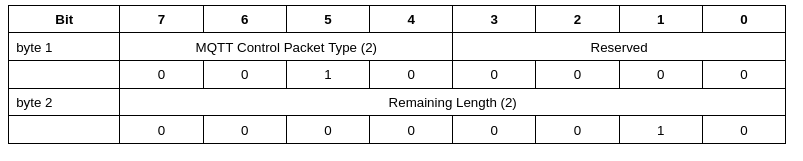
\includegraphics[width=\textwidth]{img/fixed_header_structure}
    \caption[Struktur des Fixed Headers in einem \gls{mqtt}-Paket]{Aus der Spezifikation von \gls{mqtt} Version 3.1.1~\cite{mqtt}
        zeigt die Struktur des Fixed Headers in einem \gls{mqtt}-Paket.
        Er besteht aus 2 Bytes und enthält den Steuerpakettyp (\textit{hier} 0010 für \texttt{CONNECT}) und Flags (hier \textit{Reserved})
        sowie die verbleibende Länge des Pakets.}
    \label{fig:fixed_header_structure}
\end{figure}
Der Fixed Header besteht aus drei Hauptbestandteilen~\ref{fig:fixed_header_structure}:
\begin{itemize}
    \item Steuerpakettyp: (4 Bits): MQTT definiert 14 Pakettypen (im Bereich von \texttt{0001} bis \texttt{1110}), was
    bedeutet, dass es 14 mögliche Werte für diese 4 Bits gibt
    \item Flags (4 Bits): Die Flags hängen vom Pakettyp ab, was die Anzahl der gültigen Kombinationen verringert
    \item Verbleibende Länge: Die verbleibende Länge gibt an, wie viele Bytes nach dem Fixed Header folgen
\end{itemize}
Die Spezifikation von \gls{mqtt} sieht vor, dass von den 14 möglichen Werten für den Steuerpakettyp nur 10 gültige Werte
für einen validen Steuerpakettypen existieren, die von dem Client zum Broker gesendet werden können~\cite{mqtt-fixed-header}.
Ausgegangen wird von der Generierung eines validen Connect Pakets, welches den Steuerpakettyp \texttt{CONNECT} hat.
Betrachtet wird zunächst die Wahrscheinlichkeit, dass der Fixed Header gültig ist.
Hierbei wird folgende Annahme getroffen:
\[
    P(\text{gültiger Fixed Header}) = P(\text{gültiger Steuerpakettyp}) \times P(\text{gültige Flags}) \times P(\text{gültige verbleibende Länge})
\]
Die Wahrscheinlichkeit, dass der Steuerpakettyp gültig ist, beträgt:
\[
    P(\text{gültiger Steuerpakettyp}) = \frac{M}{N} = \frac{1}{16}
\]
Wobei \textit{M} die Anzahl der gültigen Werte für den Steuerpakettyp \texttt{CONNECT} 0001 ist und \textit{N} die Anzahl der möglichen Werte, die
für die 4 Bits des Steuerpakettyps verwendet werden können.
Die Wahrscheinlichkeit, dass die Flags gültig sind, beträgt:
\[
    P(\text{gültige Flags}) = \frac{K}{N} = \frac{1}{16}
\]
Wobei \textit{K} die Anzahl der gültigen Kombinationen für die Flags ist und \textit{N} die Anzahl der möglichen Werte für die 4 Bits der Flags.
Hierbei ist zu beachten, dass die Flags bei einem \texttt{CONNECT}-Paket reserviert sind und somit nur die gültige Kombination
0000 für die Flags existieren.\newline
Das Zweite Byte des Fixed Headers enthält die verbleibende Länge des Pakets.
Die verbleibende Länge ist ein variable-length-integer, der die Anzahl der Bytes angibt, die nach dem Fixed Header folgen.
Sie kann Werte von 0 bis 127 annehmen.
Somit ergibt sich die Wahrscheinlichkeit, dass die verbleibende Länge gültig ist:
\[
    P(\text{gültige verbleibende Länge}) = \frac{128}{256}
\]
Die Wahrscheinlichkeit, dass der Fixed Header gültig ist, beträgt:
\[
    P(\text{gültiger Fixed Header}) = \frac{1}{16} \times \frac{1}{16} \times \frac{128}{256} \approx 1.938 \times 10^{-3}
\]
Der Variable Header enthält zusätzliche Informationen, die je nach Pakettyp variieren.
Für ein \texttt{CONNECT}-Paket enthält der Variable Header die Bytes für den Protokollnamen, die Protokollversion, Connect Flags
und Keep Alive.
Die Länge des Variable Headers beträgt 10 Bytes.
Die Wahrscheinlichkeit, dass der Variable Header gültig ist, beträgt:
\begin{multline}
    P(\text{gültiger Variable Header}) = P(\text{gültige Länge des Protokollnamens}) \\
    \times P(\text{gültiger Protokollnamen}) \times P(\text{gültige Protokollversion}) \times P(\text{gültige Connect Flags}) \\
    \times P(\text{gültiges Keep Alive})
\end{multline}
Die Länge des Protokollnamens ist festgelegt und beträgt 2 Bytes.
Die Wahrscheinlichkeit, dass die Länge des Protokollnamens gültig ist, beträgt:
\[
    P(\text{gültige Länge des Protokollnamens}) = \frac{1}{256} \times \frac{1}{256}
\]
\begin{figure}[H]
    \centering
    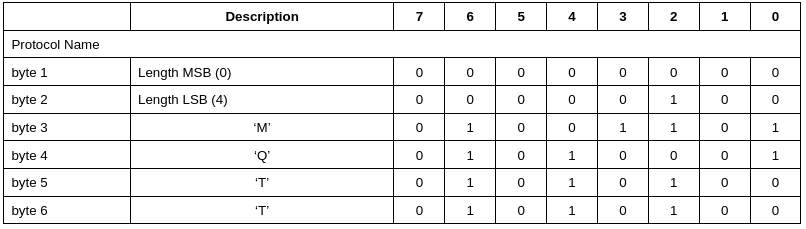
\includegraphics[width=\textwidth]{img/mqtt_prot_name}
    \caption[Struktur des Protokollnamens in einem \gls{mqtt}-Paket]{Zeigt die Struktur des Protokollnamens, entnommen aus der Spezifikation von \gls{mqtt} Version 3.1.1~\cite{mqtt-variable-header}.
        Der Protokollname ist festgelegt und muss \texttt{MQTT} sein und ist sechs Bytes lang.}
    \label{fig:mqtt_prot_name}
\end{figure}
Der Protokollname ist festgelegt auf vier Bytes und muss \texttt{MQTT} sein~\ref{fig:mqtt_prot_name}.
Aus der Struktur in der Abbildung~\ref{fig:mqtt_prot_name} ergibt sich die Wahrscheinlichkeit, dass der Protokollname gültig ist:
\[
    P(\text{gültiger Protokollname}) = \frac{1}{256}^4
\]
Zudem kommt hinzu, dass die Protokollversion festgelegt ist und \texttt{0x4} sein muss.
Die Protokollversion ist ein Byte lang und kann 256 mögliche Werte annehmen.
Somit ergibt sich die Wahrscheinlichkeit, dass die Protokollversion gültig ist:
\[
    P(\text{gültige Protokollversion}) = \frac{1}{256}
\]
Die Connect Flags sind ein Byte lang und können 256 mögliche Werte annehmen.
Die Wahrscheinlichkeit, dass die Connect Flags gültig sind, erschließt sich aus folgendem Regelwerk:
\begin{itemize}
    \item Bit 0 muss immer 0 sein
    \item Bit 1 kann 0 oder 1 sein. Wenn Bit 1 den Wert 0 hat, dann müssen die Bits 3-5 auch 0 sein
    \item Bit 2 kann 0 oder 1 sein
    \item Bit 3 und 4 können die Werte 00, 01 oder 10 annehmen, wenn Bit 1 den Wert 1 hat
    \item Bit 5 kann nur 1 sein, wenn Bit 1 den Wert 1 hat, ansonsten muss Bit 5 den Wert 0 besitzen
    \item Bit 6 und 7 können 0 oder 1 sein
\end{itemize}
Daraus ergibt sich die Wahrscheinlichkeit, dass die Connect Flags gültig sind:
\begin{equation}\label{eq:valid_connect_flags}
    P(\text{gültige Connect Flags}) = P(\text{Bit0}) \times P(\text{Bit1}) \times P(\text{Bit2}) \times P(\text{Bit3,4}) \times P(\text{Bit5}) \times P(\text{Bit6,7})
\end{equation}
\begin{itemize}
    \item Wenn Bit 2 = 0:

    \begin{itemize}
        \item Bit 3 + 4 = 00 (1 Möglichkeit)
        \item Bit 5 = 0 (1 Möglichkeit)
    \end{itemize}
\begin{multline}
    P(\text{Bit 3 + 4 + 5} \mid \text{Bit 2} = 0) = \frac{1}{8} \quad \\ \text{(es gibt 8 mögliche Kombinationen für Bit 3, 4 und 5, aber nur eine gültige)}
\end{multline}
    \item Wenn Bit 2 = 1:

    \begin{itemize}
        \item Bit 3 + 4 = 00, 01 oder 10 (3 Möglichkeiten)
        \item Bit 5 = 0 oder 1 (2 Möglichkeiten)
    \end{itemize}
\begin{multline}
    P(\text{Bit 3 + 4 + 5} \mid \text{Bit 2} = 1) = \frac{6}{8} \quad \\ \text{(es gibt 8 mögliche Kombinationen für Bit 3, 4 und 5, und 6 davon sind gültig)}
\end{multline}
\end{itemize}

\begin{multline}
    P(\text{Bit 3 + 4 + 5}) = P(\text{Bit 2} = 0) \times P(\text{Bit 3 + 4 + 5} \mid \text{Bit 2} = 0)+ P(\text{Bit 2} = 1) \times \\
    P(\text{Bit 3 + 4 + 5} \mid \text{Bit 2} = 1)
\end{multline}
\[
    P(\text{Bit 3 + 4 + 5}) = \frac{1}{2} \times \frac{1}{8}+ \frac{1}{2} \times \frac{6}{8}= \frac{1}{16}+ \frac{6}{16}= \frac{7}{16}
\]
Somit ergibt sich aus der Gleichung~\ref{eq:valid_connect_flags} die Wahrscheinlichkeit, dass die Connect Flags gültig sind:
\[
    P(\text{gültige Connect Flags}) = \frac{1}{2} \times 1 \times 1 \times \frac{7}{16} \times 1 \times 1 = \frac{7}{32}
\]
Das Keep Alive-Intervall ist ein 2-Byte-Wert, der die Zeit in Sekunden angibt, die der Client auf eine Antwort des Brokers
wartet.
Das Intervall kann Werte von 0 bis 65535 annehmen.
Die Wahrscheinlichkeit, dass das Keep Alive-Intervall gültig ist, beträgt 1, da alle Werte innerhalb der zwei Bytes zugelassen
werden.\newline
Die Wahrscheinlichkeiten für einen gültigen Variable Header sind somit:
\[
    P(\text{gültiger Variable Header}) = \left(\frac{1}{256}\right)^2 \times \left(\frac{1}{256}\right)^4 \times \frac{1}{256} \times \frac{7}{32} \times 1 \approx 3.036 \times 10^{-18}
\]
Um die Anzahl der Versuche zu berechnen, die notwendig sind, um mit einer 99-prozentigen Wahrscheinlichkeit ein gültiges
Paket mit korrekt generiertem Fixed und Variable Header zu erzeugen, wird folgende Formel verwendet:
\[
    n = \frac{\log(1 - P_{\text{Ziel}})}{\log(1 - P_{\text{Erfolg}})}
\]
Dabei beschreibt \textit{$P_{\textsubscript{Ziel}}$} die Zielwahrscheinlichkeit, dass ein gültiges Paket generiert wird, und
\textit{$P_{\textsubscript{Erfolg}}$} die Wahrscheinlichkeit, dass ein gültiger Fixed und Variable Header generiert wird.
Die Gesammtwahrscheinlichkeit für ein Paket mit einem gültigen Fixed und Variable Header beträgt:
\begin{multline}
    P(\text{Erfolg}) = P(\text{gültiger Fixed Header}) \times P(\text{gültiger Variable Header}) = \\
    1.938 \times 10^{-3} \times 3.036 \times 10^{-18} \\
    \approx 5.89 \times 10^{-21}
\end{multline}
Nun kann die Anzahl der Versuche berechnet werden, die notwendig sind, um mit einer 99-prozentigen Wahrscheinlichkeit ein
gültiges Paket zu generieren:
\[
    n = \frac{\log(1 - 0.99)}{\log(1 - 5.89 \times 10^{-21})} \approx 7.819 \times 10^{20}
\]
Bei einer gemessenen Ausführgeschwindigkeit von ca.\ 78 Paketen pro Sekunde würde es also ca. $10^{19}$ Sekunden dauern, um
mit einer Wahrscheinlichkeit von \SI{99}{\percent} ein gültiges Paket zu generieren.
Das entspricht ca.\ $3.22 \times 10^{11}$ Jahren für die Generierung eines korrekten Fixed und Variable Headers.\newline
Diese Berechnungen zeigen, dass das Fixieren von Teilen des Pakets (wie Fixed Header und Variable Header) die
Anzahl der benötigten Pakete zur Erzeugung eines gültigen Pakets erheblich reduziert.
Dies ist besonders wichtig für die Effizienz von Fuzzing-Tests, da es die Anzahl der Tests verringert, die benötigt werden,
um die gewünschten Ergebnisse zu erzielen.
\newline\newline
Durch das Fixieren bestimmter Schlüsselparameter des \gls{mqtt}-Pakets, wie dem Fixed Header und dem Topic, wird die Wahrscheinlichkeit,
dass ein gültiges Paket generiert wird, signifikant erhöht.
Dies ist besonders wichtig für effizientes Fuzzing, da es die Anzahl der möglichen ungültigen Pakete reduziert und die Effektivität der Tests steigert.
\begin{figure}[H]
    \centering
    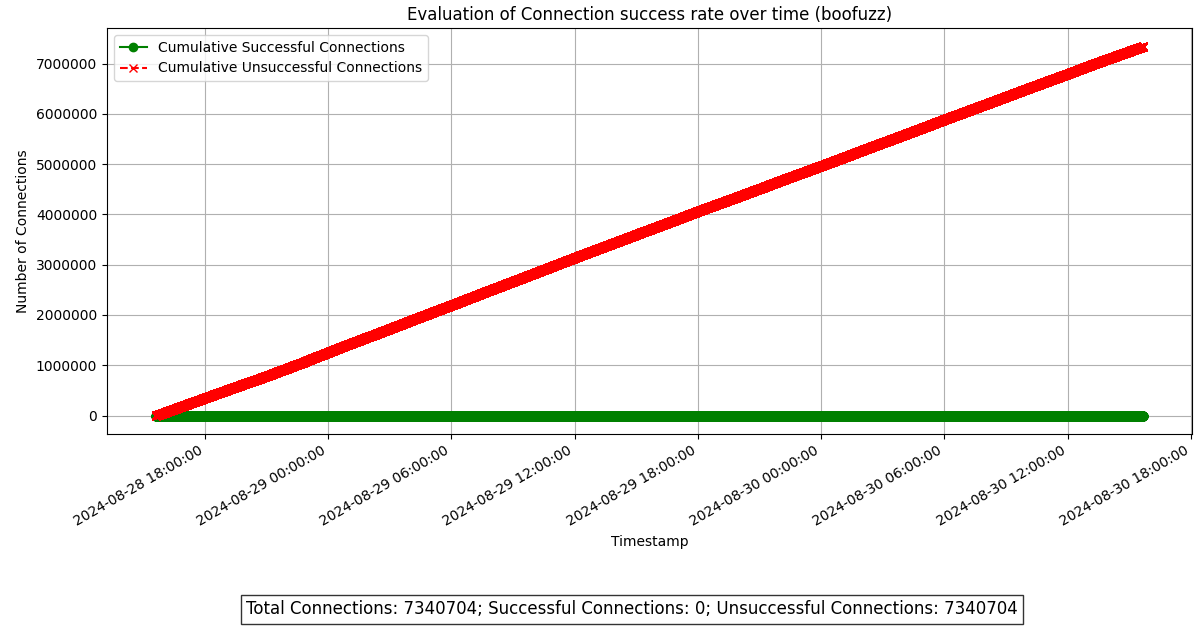
\includegraphics[width=\textwidth]{img/connection_evaluation_boofuzz}
    \caption{Vergleich der gültigen Pakete bei zufälligem Fuzzing mit boofuzz ohne statisch definierte Felder}
    \label{fig:valid_packets}
\end{figure}
\noindent Diese Grafik~\ref{fig:valid_packets} ist das Ergebnis einer Fuzzing-Kampagne, bei der über einen Zeitraum von 48 Stunden eine extrem hohe Anzahl an Verbindungsversuchen durchgeführt wurde.
Auch trotz der hohen Anzahl an Verbindungsversuchen, die in dieser Grafik dargestellt sind, konnte kein gültiges Paket generiert werden.
Das Fixieren der bereits genannten Felder führte bei einer weiteren Kampagne über 48 Stunden auch zu keinem gültigen Paket.
\begin{figure}[H]
    \centering
    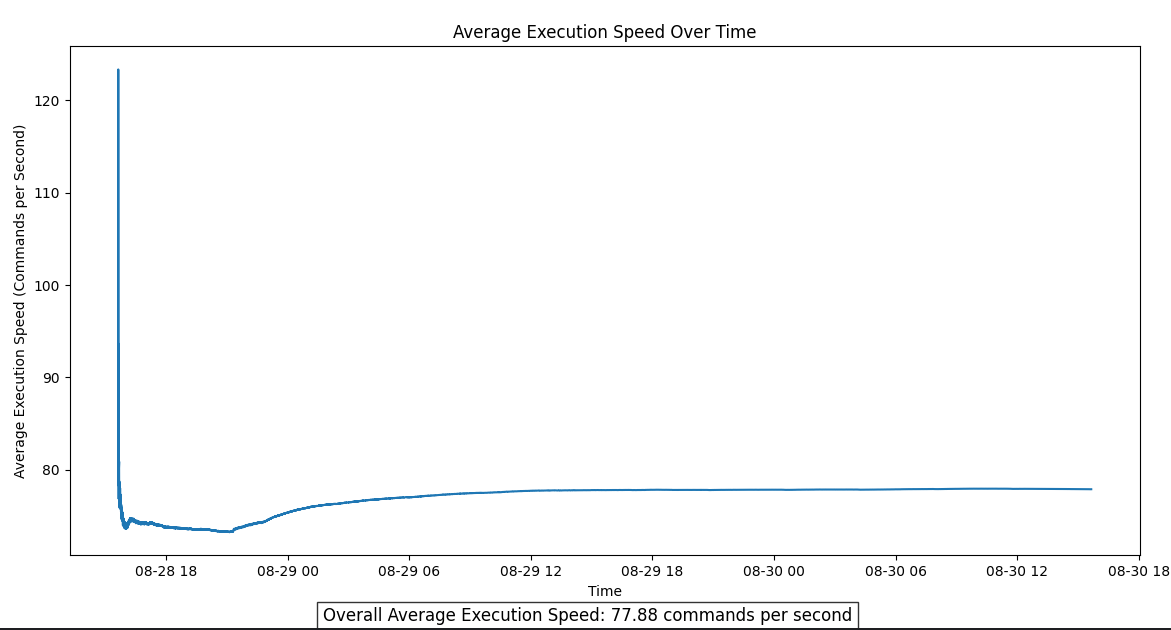
\includegraphics[width=\textwidth]{img/average_exec_speed_boofuzz_normal}
    \caption{Durchschnittliche Ausführungsgeschwindigkeit von boofuzz in einem Zeitraum von 48 Stunden}
    \label{fig:exec_speed_boo_normal}
\end{figure}
\noindent Die durchschnittliche Ausführungsgeschwindigkeit von boofuzz ist in dieser Grafik dargestellt.
In ihr ist zu erkennen, dass die Geschwindigkeit des Fuzzings über den Zeitraum von 48 Stunden relativ konstant bleibt.
Die einzige Ausnahme bildet der Anfangszeitraum der Fuzzing-Kampagne, in dem die Geschwindigkeit kurzzeitig rapide abfällt.
Dies hängt mit der Mutationsstrategie von boofuzz zusammen, die zu Beginn der Kampagne eine Vielzahl von großen Mutationen
durchführt, um das Zielsystem zu erkunden.
Zunächst wurden relativ kleine Pakete generiert, die jedoch aufgrund der geringen Wahrscheinlichkeit eines gültigen Pakets
keine Ergebnisse lieferten.
Im späteren Verlauf wurden jedoch größere Pakete generiert, was die Mutation erheblich verlangsamte.
Wichtig anzumerken ist die Strategie von boofuzz.
Trotz definition von statischen feldern im Header-Bereich wurden zufällige Bytes an den Kopf des Pakets angehängt.
Dies führte dazu, dass die Wahrscheinlichkeit eines gültigen Pakets weiterhin sehr gering war.
\begin{figure}[H]
    \centering
    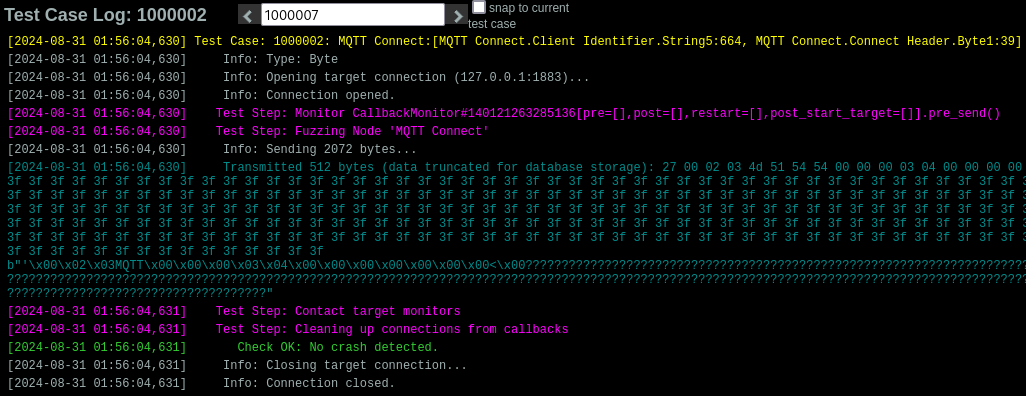
\includegraphics[width=\textwidth]{img/boofuzz_case_log}
    \caption{Diese Grafik zeigt einen Einblick zur Generierung von weiterhin ungültigen Paketen aufgrund des zufälligen Anhängens von Bytes
    im Header des Pakets.}
    \label{fig:boo_case_log}
\end{figure}
\noindent Erkennbar ist die Generierung falscher Pakete durch den festen definierten Header \texttt{0x020x03MQTT}, welcher aus der
Abbildung~\ref{fig:boo_case_log} hervorgeht.\newline\newline
Aus diesem Kapitel geht hervor, dass die Effektivität dieses Fuzzers stark von der Definition mehrerer Felder abhängt.
Im Falle von komplexeren Protokollen wie \gls{mqtt} ist es wichtig, dass eine Definition der Struktur der Felder in
der Implementierung des Fuzzers vonnöten ist, sodass die generierten Eingaben möglichst Effektiv sind.
Hierzu ist es wichtig, mehrere Aspekte des Protokolls zu definieren und zu fuzzen, um möglichst strukturiert und effektiv
an die Generierung von gültigen Paketen heranzugehen.
Dies kann in Zukunft dadurch umgesetzt werden, dass mehrere Instanzen des Fuzzers gestartet werden, die jeweils auf ein
bestimmtes Feld des \gls{mqtt}-Pakets fokussiert sind und somit die Wahrscheinlichkeit eines gültigen Pakets erhöht wird.